% Chapter Template

\chapter{Summary of Chapter 6: Web portal} % Main chapter title
\label{chapter-webportal}

%----------------------------------------------------------------------------------------
%	SECTION 1
%----------------------------------------------------------------------------------------

Under \href{http://openbiodiv.net}{\url{openbiodiv.net}} one can reach the main portal giving access to OpenBiodiv resources. This portal was developed by Pensoft to support OpenBiodiv. \href{http://openbiodiv.net}{OpenBiodiv.net} presents two visual elements to the user: the search bar and list of application icons in the bottom. Furthermore, under \href{http://graph.openbiodiv.net}{\url{graph.openbiodiv.net}} (also accessible from the icon SPARQL endpoint) one can reach the OpenBiodiv workbench, a feature of GraphDB that gives web access to the SPARQL endpoint.

These User Interface (UI) features are designed to facilitate the three user types of the system that we envisage:

\begin{enumerate}
    \item Basic level: uses search bar.
    \item Specialist level: uses apps.
    \item Power user: uses the work-bench of the system or R.
\end{enumerate}

\section{Functionality of the system}

In this section we discuss how every user-type can use the system.

\subsection{Basic usage}

The basic level of interaction is for users who want a quick look into the system's database; they can be beginners without knowledge of the Semantic Web or of taxonomy, or advanced users with little time or a very basic query. An example of such a user will simply look for an entity (e.g. taxonomic name, person) and would like to retrieve some information about it. 

\begin{figure}
\centering
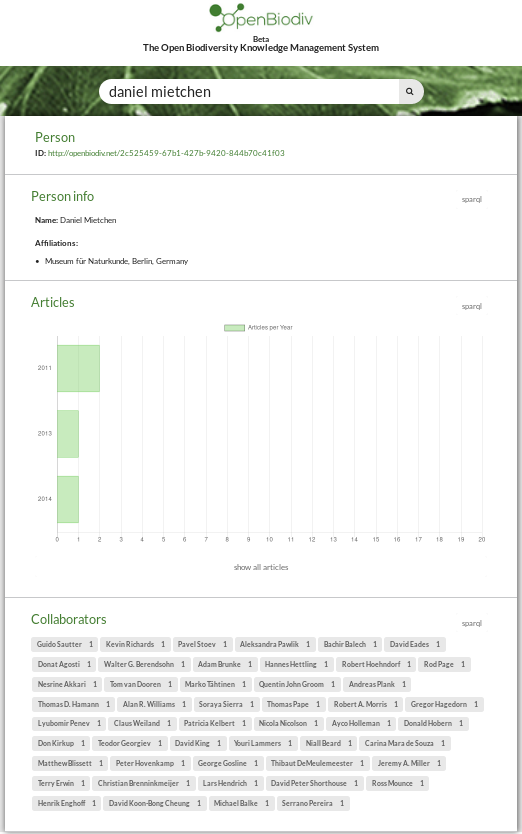
\includegraphics[width=\textwidth]{Figures/basic-level.png}
\decoRule
\caption{Illustration of basic usage of OpenBiodiv to look information about a person.}
\label{fig:basic-level}
\end{figure}

\subsection{Specialist level}

A specialist is someone who has a question of particular taxonomic importance that cannot be answered by a simple name-based look-up. For example, a collection manager at a museum may want to periodically check for articles that make use of their collection in order to justify additional funding to prevent natural disasters. Or a taxonomist interested in a particular region or group may want to stay up to date with published literature fitting those criteria---let's say weevils (Curculionidae) of Arizona, U.S.A. 

\subsection{Power user}

The power user is someone with knowledge of the Semantic Web and its technologies (SPARQL, ontologies, etc.). The power user goes to the workbench and executes their queries there, or uses the functionality of the RDF4R package described in Chapter~\ref{chapter-rdf4r} to execute SPARQL directly on the OpenBiodiv endpoint directly from the R environemnt.

\section{Implementation}

The UI-components of the web portal are developed in the ReactJS JavaScript framework written by Facebook. Server-side processing is done in PHP. This part of OpenBiodiv is not open source and cannot be discussed in detail in the present dissertation effort.
